\section{Fourier transform}

\subsection{Gaussian kernel in Fourier space}

\newcommand{\F}[1]{\mathcal F\left\{#1\right\}}
% \paragraph{Convolution using Fourier transformation in general}~\smallskip

By the convolution theorem, the convolution $(f \ast g)$ of two functions (or
signals or images) $f$ and $g$ can in general be performed using Fourier
transformation as such: $f \ast g = \mathcal
F^{-1}\{\F{f} * \F{g}\}$. In Python, this can be implemented for signals
\texttt{X} and \texttt{Y} as \texttt{ifft(fft(X) * fft(Y))}.

Below snippet shows my code for Gaussian filtering using convolution in Fourier
space, using a Gaussian kernel constructured directly in Fourier space:

\begin{minted}[linenos=true]{python}
def scale_fft(img, sigma):
    n, m = s = np.asarray(img.shape)
    X, Y = ifftshift(np.indices(s), axes = (1, 2))

    # compute sigma for the frequency domain.
    sigma_X, sigma_Y = s / (2 * np.pi * sigma)
    F_gauss = np.exp(-((X - n // 2) ** 2 / (2 * sigma_X ** 2) +
                       (Y - m // 2) ** 2 / (2 * sigma_Y ** 2)))
    return ifft2(fft2(img) * F_gauss).real
\end{minted}

Note line 3, where the sigma for each dimension is computed relative to the size
of that dimension, and line 5, where \texttt{ifftshift} is used to shift the
grid of indices, since the Gaussian kernel should not be centered at the middle
of the array when multiplying with the FFT of the image.


\Cref{fig:2.1} shows examples of the function for various values of $\sigma$.
\begin{figure}[H]
    \centering
    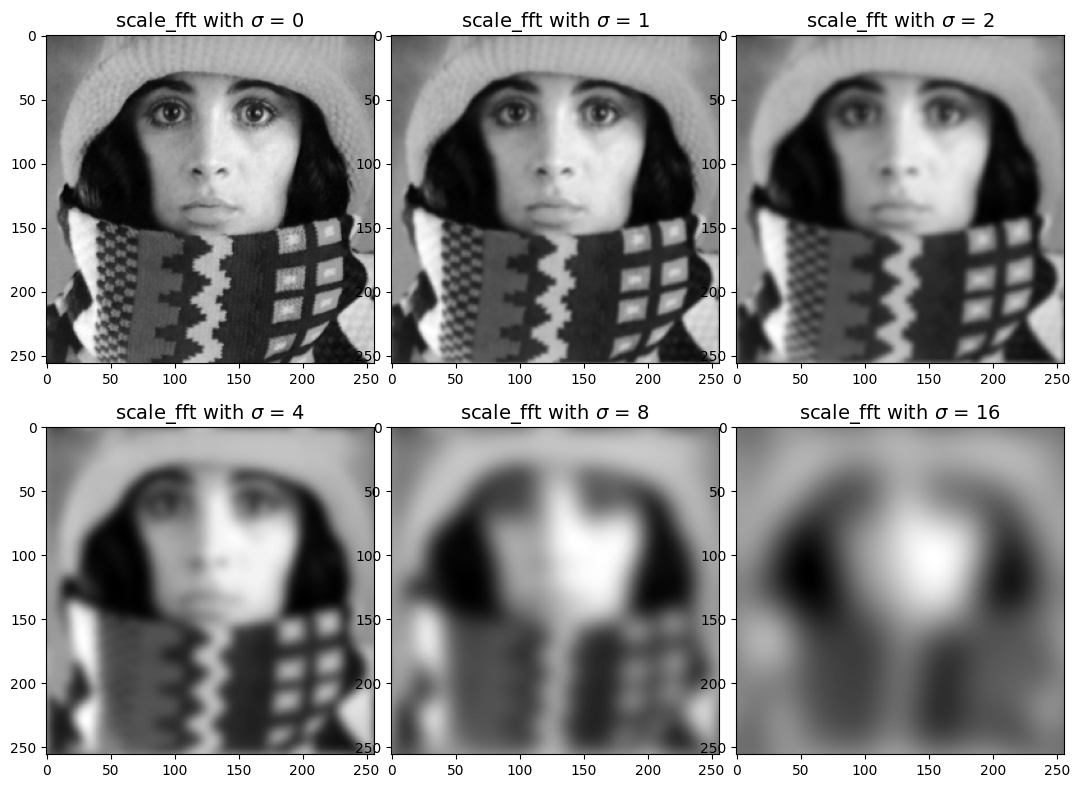
\includegraphics[width=0.7\textwidth]{figures/task_2_1.png}
    \caption{\texttt{scale\_fft} of \texttt{trui.png} for various values of
    $\sigma$.}
    \label{fig:2.1}
\end{figure}



